\subsection{Problem Formulation}
Given $N$ RGB images $\{\mathbf{I}_i\}_{i=1}^N$ of a scene and a text query $\mathcal{T}$ (e.g., ``the red mug''), our goal is to predict:
\begin{enumerate}[nosep,leftmargin=*]
    \item Per-view binary masks $\{\mathbf{M}_i \in \{0,1\}^{H \times W}\}_{i=1}^N$
    \item A world-frame 3D centroid $\mathbf{c} \in \mathbb{R}^3$ localizing the queried object
\end{enumerate}


We do \textbf{not} require ground-truth camera intrinsics or extrinsics. Prior multi-view methods assume calibrated cameras~\cite{mvsam}, while TrianguLang uses \emph{predicted} geometry from DA3-NESTED~\cite{da3}, which jointly estimates metric depth, intrinsics, and extrinsics from the input images alone. This enables deployment on uncalibrated camera systems and multi-camera setups without requiring SLAM or structure-from-motion (SfM) preprocessing.

Unlike prior work that requires per-view text prompts or click supervision, TrianguLang operates in a \emph{single-prompt} setting: the language query is provided once and propagated across all views through geometric reasoning, reducing user effort from $O(N)$ clicks to $O(1)$ text input. While recent approaches to spatial language understanding (e.g., SpatialVLM~\cite{spatialvlm}, 3D-LLM~\cite{3dllm}, LEO~\cite{leo}) require large language models or multi-step agent pipelines to interpret queries like 'nearest chair' or `mug to the left of the keyboard,' TrianguLang resolves spatial relations \textit{directly} via depth-derived 3D geometry, eliminating LLM inference latency and enabling real-time spatial grounding.


% Rather than trusting semantic similarity alone, we use geometry as a sanity check, ensuring that two pixels should only correspond if they are both semantically similar AND geometrically proximate.

\subsection{Architecture Overview}
\begin{figure}[htbp]
\centering
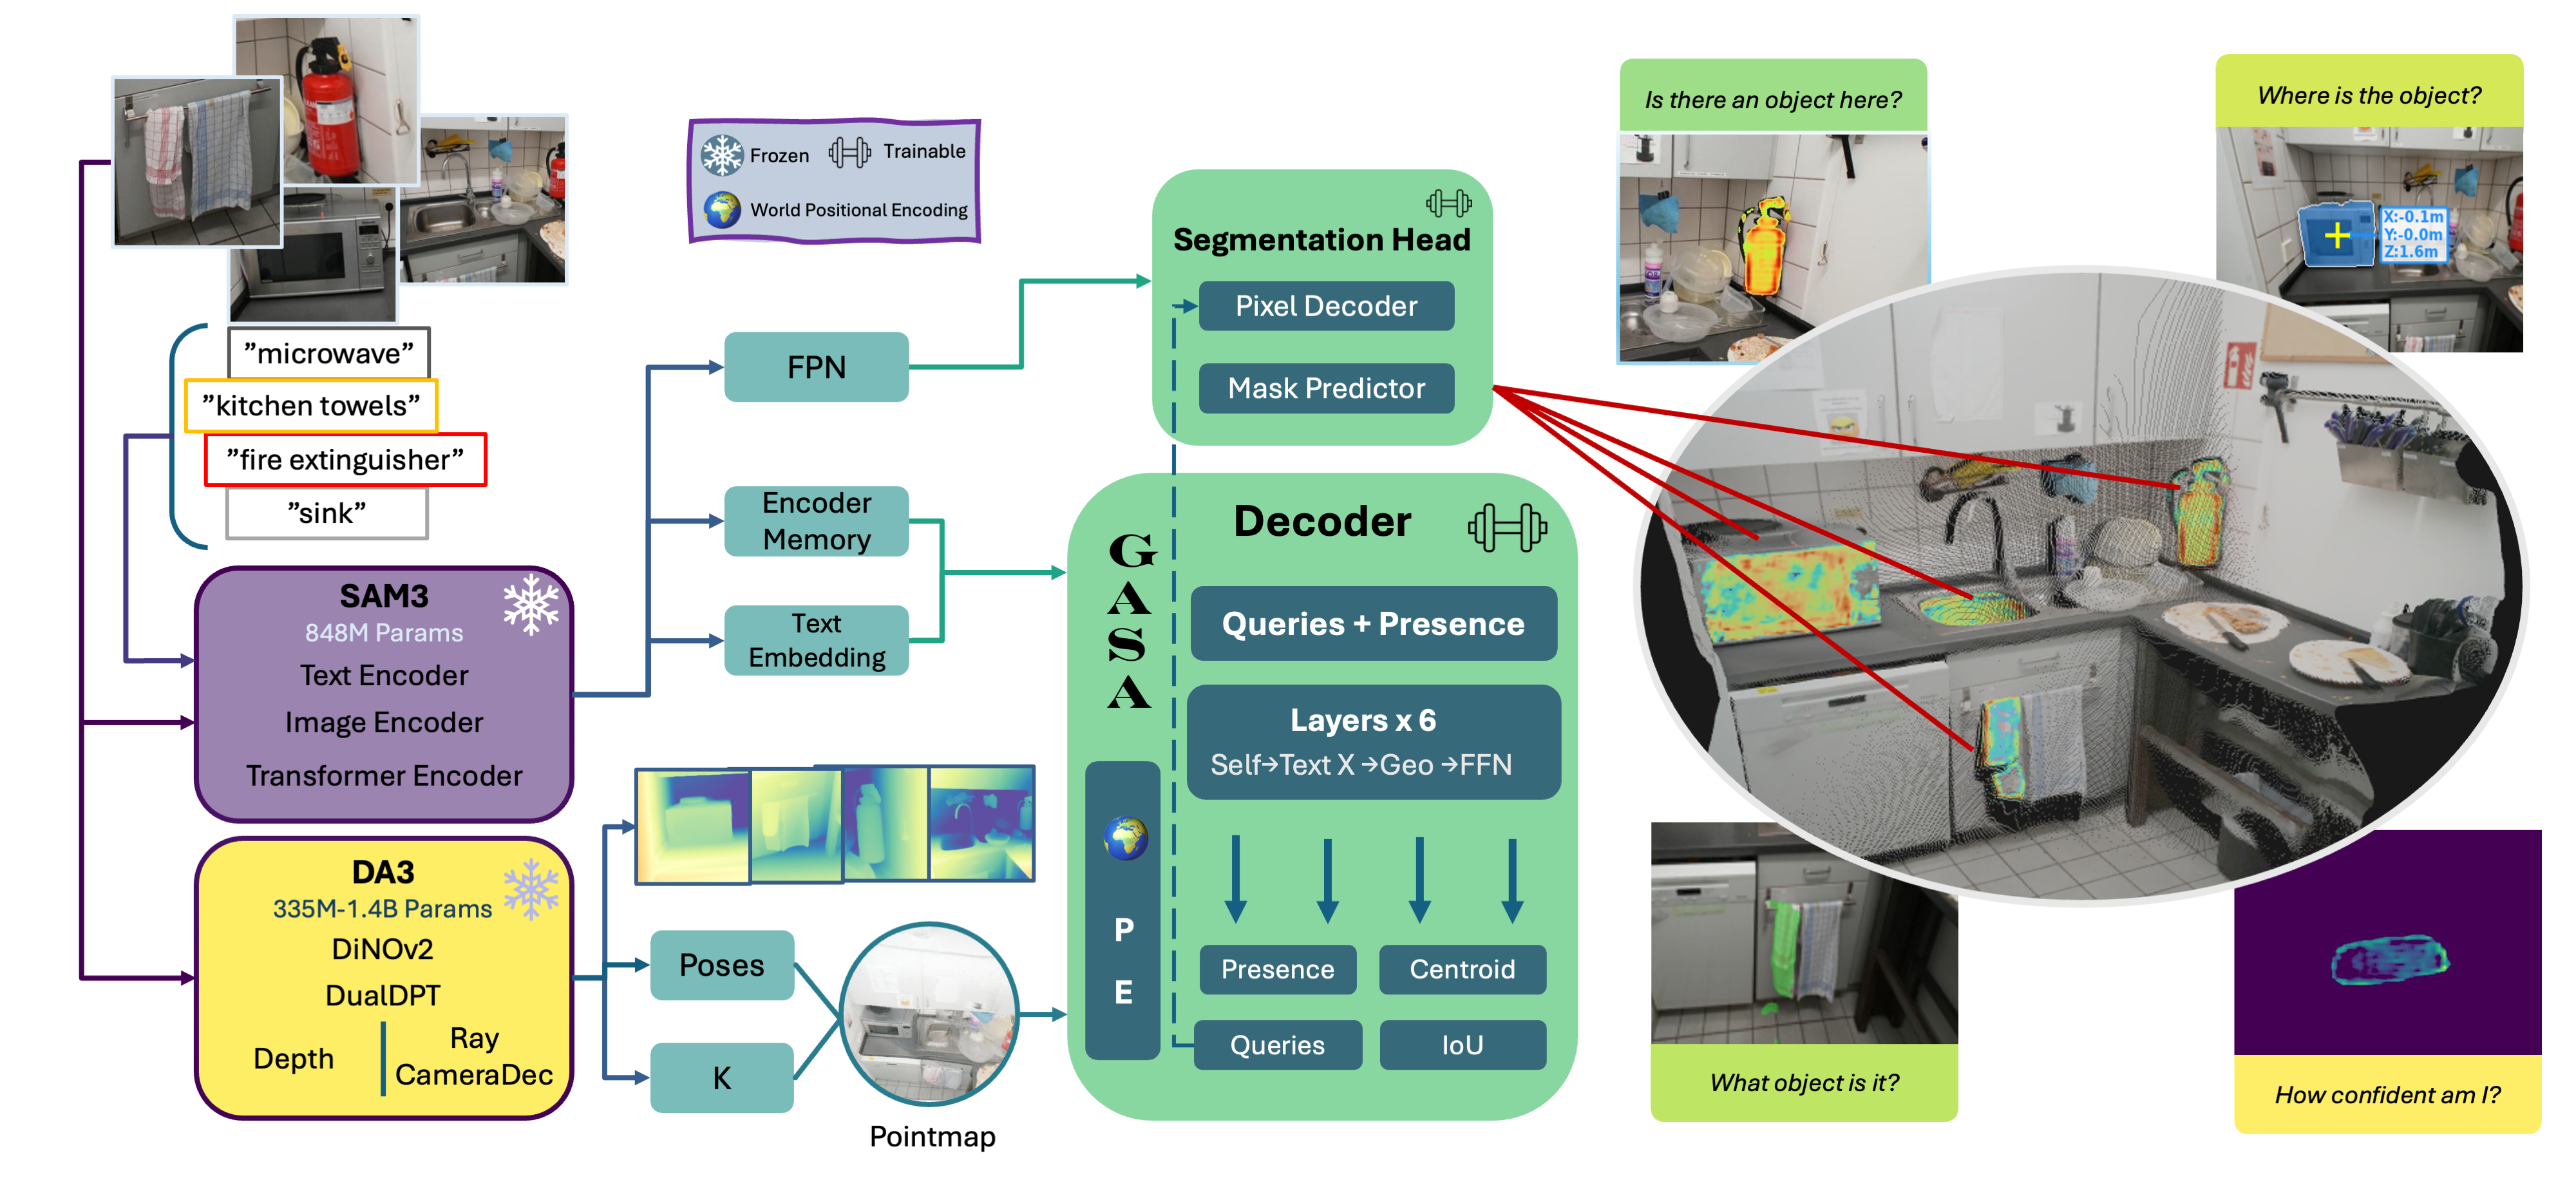
\includegraphics[width=\columnwidth]{figures/architecture_full.png}
\caption{Overview of the TrianguLang architecture}
\label{fig:arch}
\end{figure}
Figure~\ref{fig:arch} illustrates the TrianguLang architecture.

% Images are processed through two frozen foundation models: SAM3 for semantic features and DA3 for depth and pose estimation. The resulting features and pointmaps are combined through our GASA encoder/decoder, followed by a symmetric centroid head that outputs the final 3D coordinates. %

TrianguLang comprises three components (Figure~\ref{fig:arch}):
\begin{enumerate}[nosep,leftmargin=*]
    \item \textbf{SAM3 backbone} (frozen, 848M): Text-conditioned semantic features
    \item \textbf{DA3-NESTED depth model} (frozen, 1.4B): State-of-the-art metric depth and pose estimation~\cite{da3}. While other visual geometry models (VGMs) such as DUST3R~\cite{dust3r} and $\pi^3$~\cite{pi3} provide pointmaps and relative pose, DA3 additionally outputs \emph{metric} depth calibrated in meters, which is essential for accurate 3D localization and the distance-based GASA kernel.
    \item \textbf{GASA decoder} (trained, 13.7M): Geometry-aware cross-view fusion
%     \item \textbf{Centroid head} (trained): Direct 3D localization
% \todo[inline]{Centroid head or Segmentation head?}
\end{enumerate}

% \subsubsection{Frozen Backbones.}
% We leverage two pretrained foundation models:
% \begin{itemize}[nosep,leftmargin=*]
%     \item \textbf{SAM3}~\cite{sam3}: A grounded segmentation model providing text-conditioned encoder features $\mathbf{F} \in \mathbb{R}^{B \times L \times D}$ where $L = H' \times W'$ and $D = 256$.
%     \item \textbf{DA3}~\cite{da3}: Depth Anything V3 with two deployment modes:
%     \begin{itemize}[nosep,leftmargin=*]
%         \item \textit{DA3NESTED-GIANT-LARGE} (1.4B params): Jointly processes multiple views with cross-view attention, estimating metric depth $\mathbf{D}_i \in \mathbb{R}^{H \times W}$, camera intrinsics $\mathbf{K}_i \in \mathbb{R}^{3 \times 3}$, and extrinsics $\mathbf{T}_i \in SE(3)$ via ray-based pose estimation.
%         \item \textit{DA3METRIC-LARGE} (0.35B params): Monocular metric depth for real-time inference when camera-relative localization suffices.
%     \end{itemize}
% \end{itemize}


\subsection{World-Space Positional Encoding}

Standard 2D positional encodings fail to capture cross-view relationships: the same 3D point projects to different pixel coordinates across views. We address this with \textbf{world-space positional encoding} that assigns identical embeddings to the same 3D location regardless of viewpoint.

For each pixel $(u, v)$ in view $i$, we compute its 3D coordinate using DA3-estimated depth $\mathbf{D}_i$ and camera parameters:
\begin{equation}
\mathbf{P}_i(u,v) = \mathbf{T}_i \cdot \left( \mathbf{D}_i(u,v) \cdot \mathbf{K}_i^{-1} \begin{bmatrix} u \\ v \\ 1 \end{bmatrix} \right)
\label{eq:unproject}
\end{equation}
where $\mathbf{K}_i \in \mathbb{R}^{3\times3}$ denotes camera intrinsics and $\mathbf{T}_i \in SE(3)$ denotes the camera extrinsic transformation. DA3-NESTED-GIANT-LARGE jointly estimates both $\mathbf{K}_i$ and $\mathbf{T}_i$ from image features via a learned camera decoder (predicting field-of-view and relative pose), placing all views in a shared world frame \emph{without ground-truth calibration}. This is used at both training and inference time. Following NeRF~\cite{nerf}, we encode 3D coordinates with sinusoidal positional encoding projected via MLP to $D=256$.


\subsection{Geometry-Aware Semantic Attention (GASA)}
\label{sec:gasa}

Standard cross-attention matches features based purely on semantic similarity, leading to false correspondences between visually similar but geometrically distant regions (e.g., two identical mugs). GASA introduces an explicit \textbf{geometric veto} mechanism.

\subsubsection{Attention with Geometric Bias.}
GASA augments self-attention among encoder feature tokens with a geometric bias derived from their 3D positions (Eq.~\cref{eq:unproject}). Each encoder token has a known 3D position from depth unprojection; for tokens at positions $\mathbf{P}_Q$ and $\mathbf{P}_K$:
\begin{equation}
\small
\text{Attn}(\mathbf{Q}, \mathbf{K}, \mathbf{V}) = \text{softmax}\left( \frac{\mathbf{Q}\mathbf{K}^\top}{\sqrt{d}} + \beta \cdot \phi(\|\mathbf{P}_Q - \mathbf{P}_K\|_2) \right) \mathbf{V}
\label{eq:gasa}
\end{equation}
where $\beta$ is a learnable scalar and $\phi$ is a learned distance kernel. The distance $\|\mathbf{P}_Q - \mathbf{P}_K\|_2$ is computed in meters from DA3-estimated pointmaps. The kernel outputs strongly negative values for large distances. Learnable mask queries subsequently cross-attend to these GASA-refined encoder features.

\paragraph{Distance kernel $\phi$.} We parameterize $\phi$ as a 2-layer MLP with hidden dimension 32, initialized to approximate $-\log(1 + d)$. This learned kernel can adapt its distance sensitivity during training, unlike fixed-form alternatives such as RBF kernels $\phi_{\text{rbf}}(d) = -d^2 / 2\sigma^2$ or linear decay $\phi_{\text{lin}}(d) = -d$. We ablate these choices in Table~\ref{tab:ablation}; the learned kernel consistently outperforms fixed alternatives, suggesting that the optimal distance-to-bias mapping is task-dependent and benefits from end-to-end learning.


% \begin{figure}[t]
% \centering
% \fbox{\parbox{0.95\columnwidth}{\centering
% \vspace{1.5cm}
% \textbf{[Figure: GASA attention visualization]}\\[2mm]
% \small (a) Standard attention: both mugs attend\\
% (b) GASA: distant mug suppressed by $\phi(d) \ll 0$
% \vspace{1.5cm}
% }}
% \caption{GASA geometric veto. Standard attention attends to both semantically similar mugs. GASA's geometric bias suppresses the distant mug, focusing on the geometrically consistent target.}
% \label{fig:gasa}
% \end{figure}

\subsubsection{Decoder Architecture}
The GASA decoder consists of 6 transformer layers, each containing: (1) self-attention among queries, (2) text cross-attention (per-layer, following SAM3), (3) GASA cross-attention with geometric bias, and (4) feed-forward network. See Appendix~\cref{app:architecture} for details.

\begin{figure}[ht]
\begin{center}
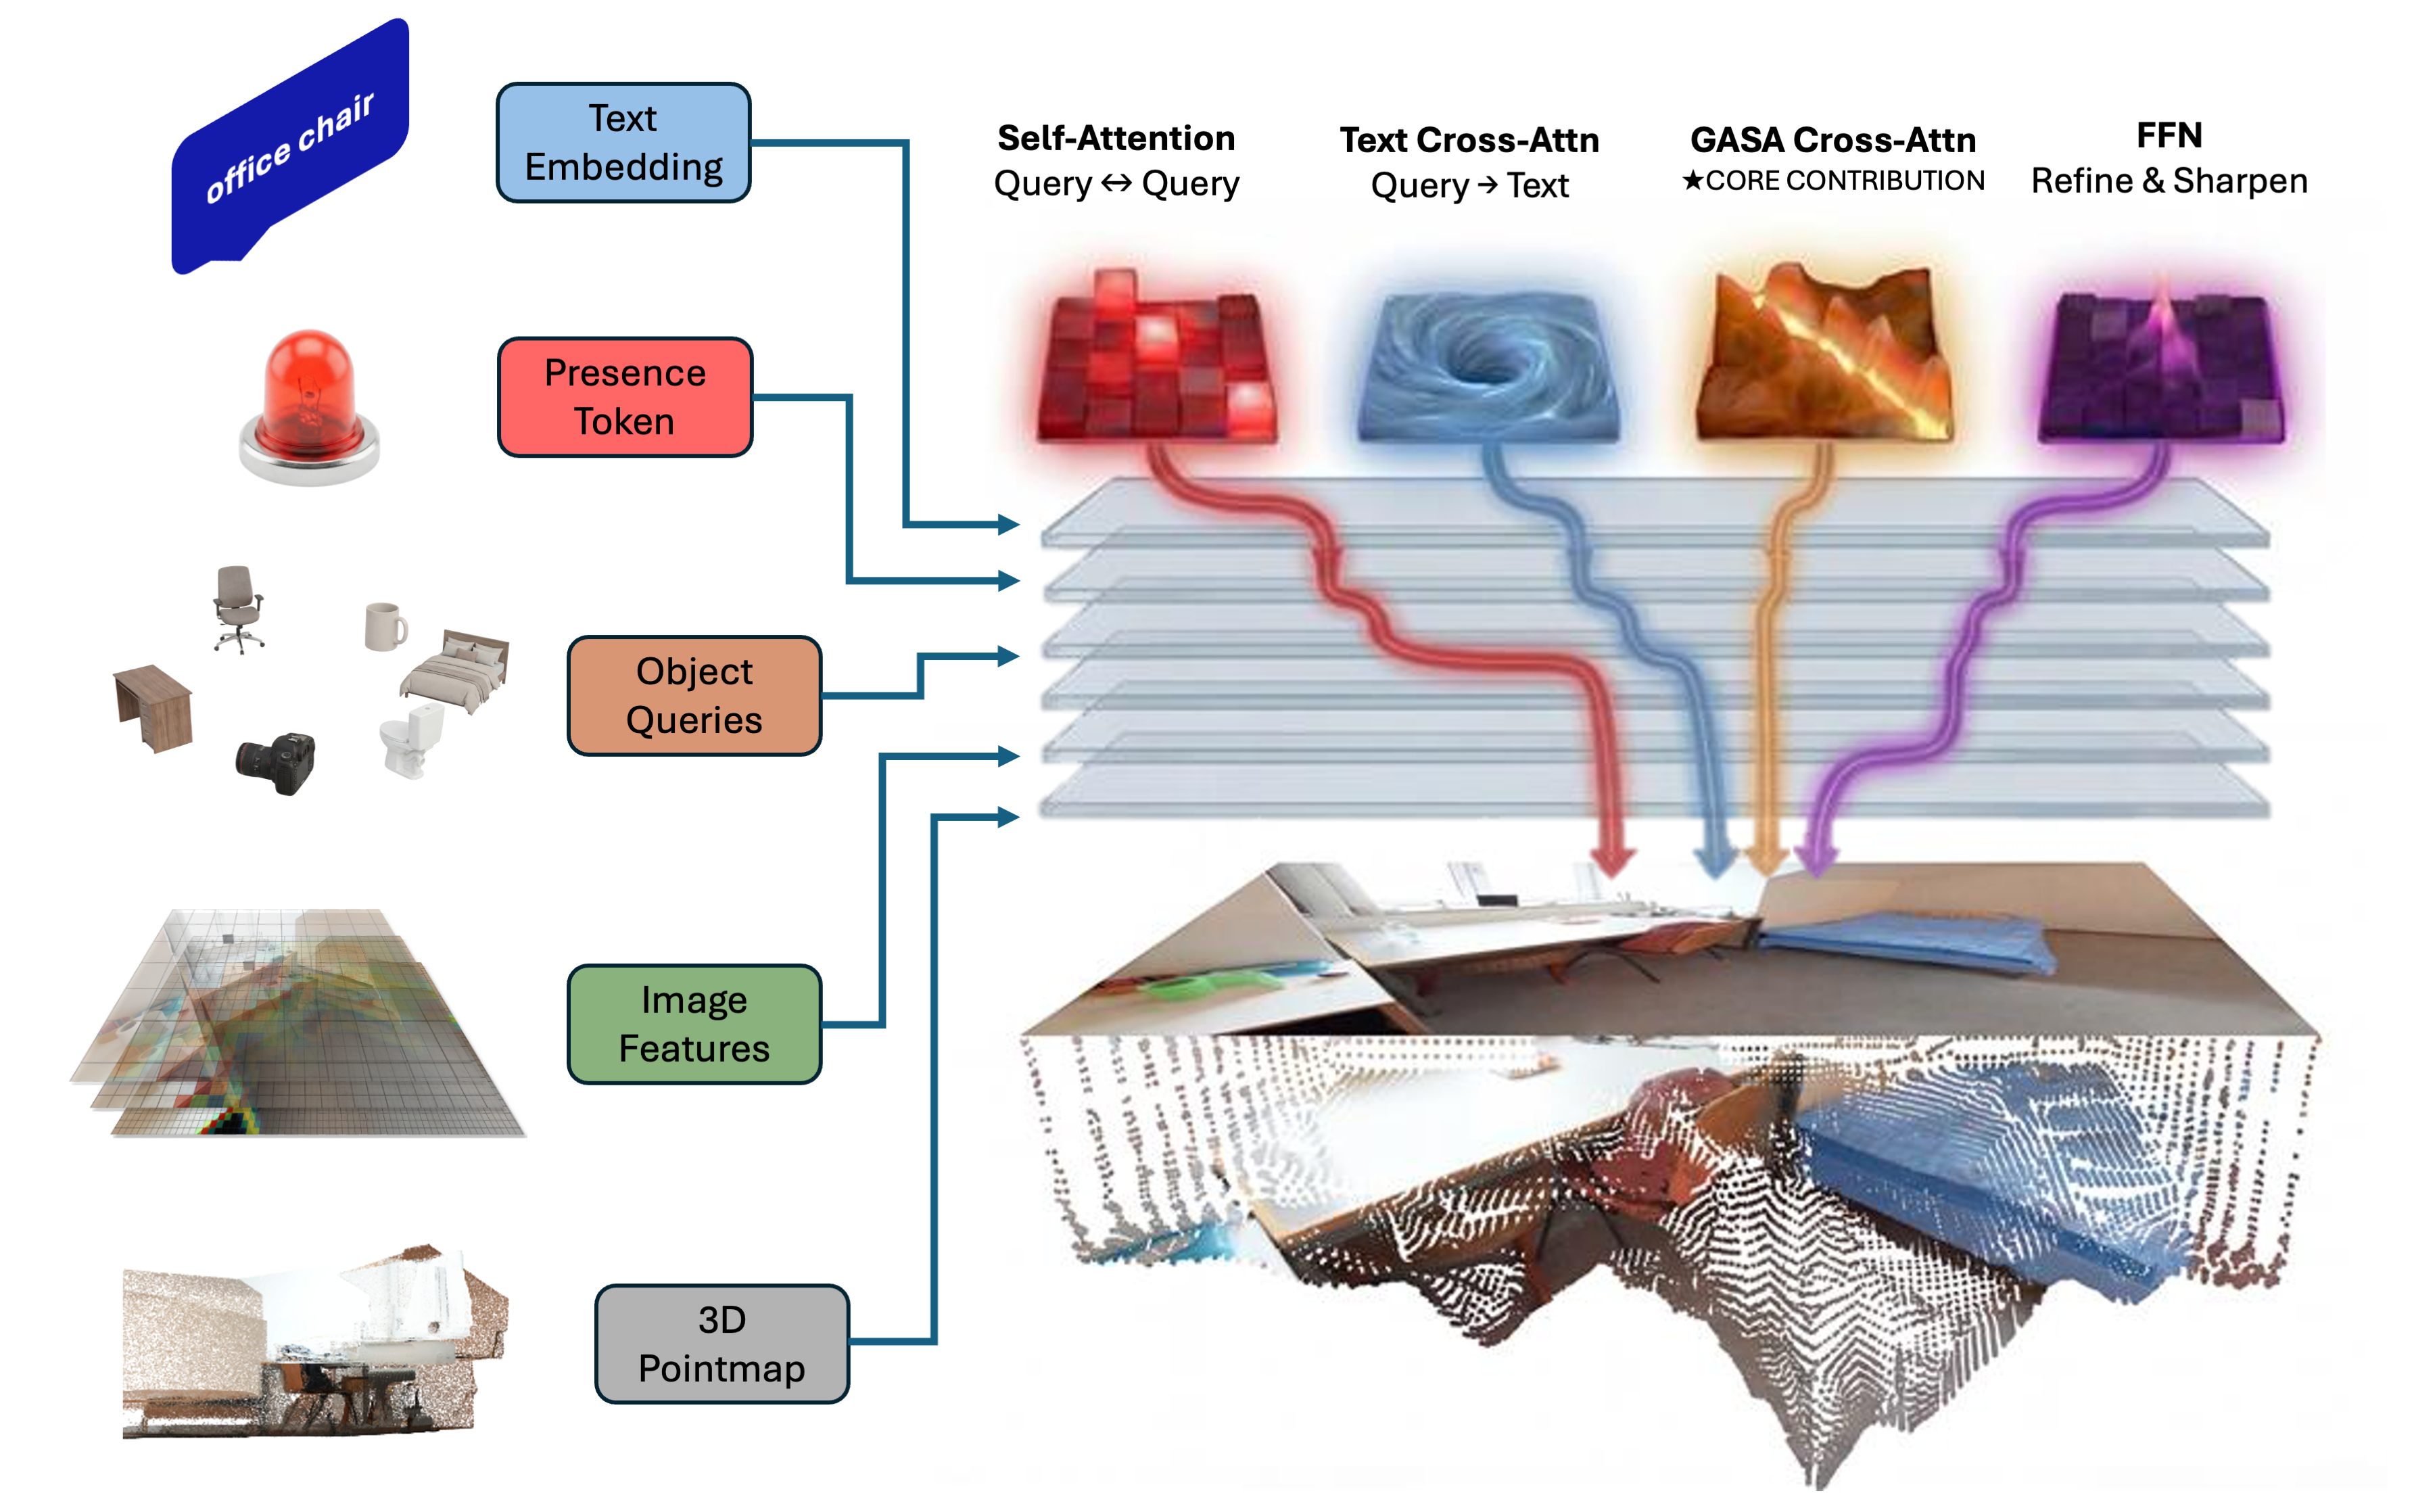
\includegraphics[width=\linewidth]{figures/decoder.png}
\end{center}
\caption{Overview of the GASA decoder. }
\label{fig:decoder}
\end{figure}


% The same physical point receives \emph{identical} positional encoding regardless of which camera observes it:
% % \begin{equation}
% %     P_i(u_i, v_i) = P_j(u_j, v_j) = \mathbf{p} \implies \text{PE}(P_i(u_i, v_i)) = \text{PE}(P_j(u_j, v_j))
% % \end{equation}
% This enables the decoder to reason about 3D consistency without explicit correspondence supervision.

% \subsection{Sheaf Consistency Loss}
% \label{sec:sheaf}
%
% To enforce cross-view coherence, we introduce a consistency loss derived from the cellular sheaf Laplacian~\cite{currysheaf,sheafnn}. We model multi-view segmentation as a sheaf $\mathcal{F}$ over a view graph, where restriction maps $\mathcal{F}_{v_i \trianglelefteq e_{ij}}$ transform per-view features to a shared comparison space via geometry-gated projections:
% \begin{equation}
% \mathcal{F}_{v_i \trianglelefteq e_{ij}}(\mathbf{f}_i, \mathbf{g}_i) = W \mathbf{f}_i \odot \sigma(\text{Gate}(\mathbf{g}_i))
% \label{eq:restriction}
% \end{equation}
% where $\mathbf{g}_i$ encodes geometric context (depth, viewing angle, edge proximity) and $\text{Gate}$ learns to down-weight unreliable correspondences. The consistency loss penalizes disagreement at 3D-corresponding pixels:
% \begin{equation}
% \mathcal{L}_{\text{sheaf}} = \frac{1}{|E|} \sum_{e_{ij}} \frac{1}{|\mathcal{C}_{ij}|} \sum_{(\mathbf{u}_i, \mathbf{u}_j) \in \mathcal{C}_{ij}} \left\| \mathcal{F}_{v_i \trianglelefteq e_{ij}}(\mathbf{f}_i, \mathbf{g}_i) - \mathcal{F}_{v_j \trianglelefteq e_{ij}}(\mathbf{f}_j, \mathbf{g}_j) \right\|_2^2
% \label{eq:sheaf}
% \end{equation}
% where $\mathcal{C}_{ij}$ are pixel correspondences with 3D distance $<10$cm from DA3 pointmaps. GASA and sheaf loss are complementary: GASA gates attention during inference; sheaf loss supervises correspondence consistency during training.

\subsection{3D Localization}
\label{sec:centroid}

Beyond 2D segmentation, TrianguLang directly predicts 3D object centroids via mask-weighted depth unprojection. For each view $i$:
\begin{equation}
\mathbf{c}_i = \frac{\sum_{u,v} \hat{M}_i(u,v) \cdot \mathbf{P}_i(u,v)}{\sum_{u,v} \hat{M}_i(u,v) + \epsilon}
\label{eq:centroid}
\end{equation}
where $\hat{M}_i \in [0,1]^{H \times W}$ is the predicted mask probability (after sigmoid) for view $i$ and $\mathbf{P}_i$ are DA3-estimated 3D coordinates (Eq.~\cref{eq:unproject}). The final centroid is selected from the view with the highest mask confidence score. The localization pipeline operates entirely on DA3-NESTED estimates, producing 3D coordinates in the estimated world frame.

\subsection{Training Objective}

The complete loss combines segmentation, ranking, and localization terms:
\begin{equation}
\mathcal{L} = \mathcal{L}_{\text{seg}} + \mathcal{L}_{\text{rank}} + \mathcal{L}_{\text{loc}}
\label{eq:total_loss}
\end{equation}

\begin{itemize}[nosep,leftmargin=*]
    \item $\mathcal{L}_{\text{seg}}$: Focal + Dice loss for mask prediction
    \item $\mathcal{L}_{\text{rank}}$: Align loss~\cite{align2024} for confidence-calibrated mask scoring plus contrastive ranking loss for correct mask ordering
    \item $\mathcal{L}_{\text{loc}}$: Smooth L1 centroid regression and binary cross-entropy presence loss for object existence prediction
\end{itemize}

See Appendix~\cref{app:loss} for detailed loss formulations and hyperparameters.

\subsection{Spatial Language Understanding}
\label{sec:spatial}

TrianguLang supports spatial qualifiers (``nearest chair'') and relational queries (``mug left of keyboard'') via geometric computation on depth-derived 3D positions, \textbf{without LLM inference}. The pipeline parses spatial keywords, generates mask candidates via SAM3, computes 3D centroids via depth unprojection, and selects the candidate satisfying the spatial constraint (e.g., $\arg\min_i d_i$ for ``nearest''). During training, we augment labels with spatial qualifiers ($p{=}0.3$) for multi-instance scenes. This enables $\sim$100ms spatial grounding vs.\ 1 to 10+ seconds for LLM-based methods~\cite{spatialvlm,3dllm,leo}. See Appendix~\cref{app:spatial} for details.
